\chapter{配管6D姿勢推定}
本章では、配管6D姿勢推定の手法について解説する。
6D姿勢推定とは、3次元空間内で物体の位置と姿勢を推定する技術であり、深層学習の活用によりその効率と精度を大幅に向上させることが可能である。
本研究では、RGB画像のみを用いる手法と、RGB-D画像を活用した手法の2種類について、それぞれの特徴と利点を述べる。


\section{検出クラス}
深層学習による画像認識では、検出対象となるオブジェクトを明確に定義することが重要である。
検出対象のオブジェクトの名前はクラスと呼ばれ、それぞれのクラスに応じた学習が行われるのが一般的である。
本研究では、配管設備のアイソメ図を効率的に作成するために、配管の構造的特徴を活用した手法を提案する。

\begin{figure}[htbt]
	\centering
	 \includegraphics[height=52mm]{Figure/detect_class.eps}
	 \caption{配管構造の例}
	 \label{fig:f1}
\end{figure}

図\ref{fig:f1}に示すように、一般的な配管は直管を中心とし、接続部分として両端に曲管やT字管が存在する。
この特性を利用し、本研究では直管を検出対象から除外し、接続部である曲管およびT字管の姿勢を推定する手法を採用した。
これにより、接続部同士のペアを直線で結ぶことで効率的にアイソメ図を描画することが可能である。

さらに、直管を検出対象に含める場合、配管設備が大規模になるにつれて認識精度が低下することが問題となる。
その主な要因は、オクルージョン(視界遮蔽)の発生である。
オクルージョンとは、前方の配管が後方の配管を隠してしまう現象であり、特に直管が多い場合には特に認識が困難になる。

以上の理由から、本研究では検出対象のクラスを曲管とT字管の2種類に限定した。
配管全体を解析するのではなく、これらの接続部に特化するアプローチを取ることで、配管構造を効率的かつ正確に解析する手法を実現する。


\section{RGB画像に基づく配管6D姿勢推定}
\section{全体構成}
RGB画像を用いた配管の6D姿勢推定には、Gen6Dを用いて実装する。
図\ref{fig:f2}にGen6Dによる6D姿勢推定の流れを示す。
\begin{figure}[htbt]
	\centering
	 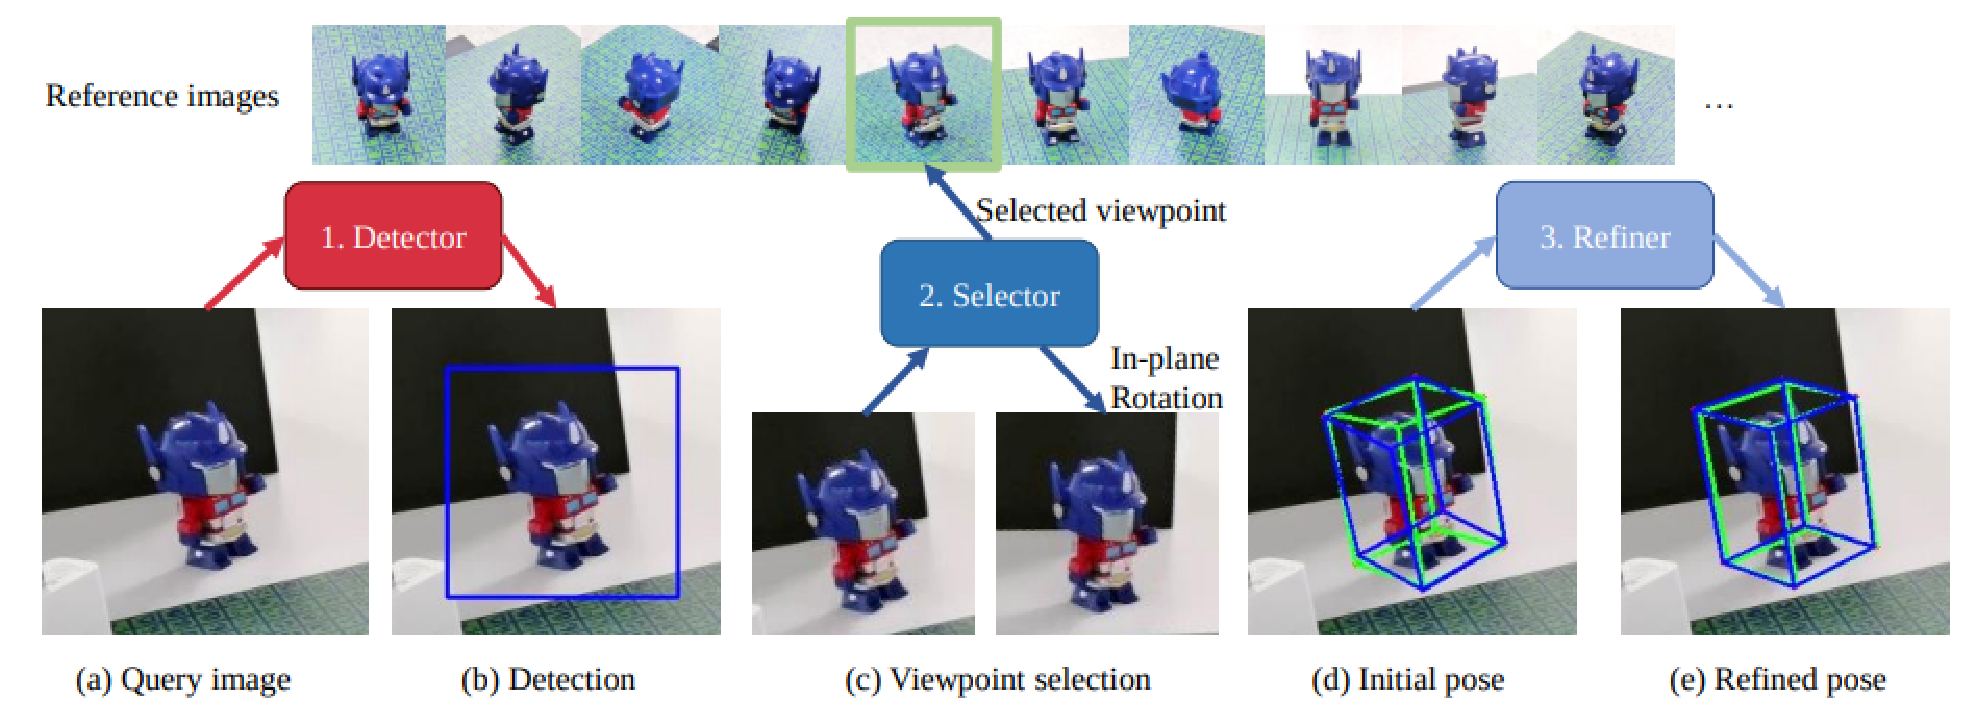
\includegraphics[height=45mm]{Figure/Gen6D.eps}
	 \caption{Gen6Dの姿勢推定方法の流れ}
	 \label{fig:f2}
\end{figure}

Gen6Dは物体検出、画像マッチング、姿勢補正の3つのステップから構成されている。
物体検出、画像マッチング、姿勢補正の3つのステップで構成されている。
物体検出では、入力画像から対象物体の領域を検出し、画像マッチングでは、検出された領域を参照画像と比較して最も類似する視点を持つ画像を選択する。
姿勢補正では、初期姿勢を基に、物体の6D姿勢をさらに精度良く推定する。

しかし、Gen6Dは単一物体の姿勢推定に特化しており、複数物体を同時に処理することが困難である。
このため、複数の配管部品を含むアイソメ図を作成する際には、複数物体を同時に検出可能な手法が求められる。
一方で、YOLOは各検出クラスに対して複数物体の検出が可能であり、Gen6Dの物体検出ステップの代替手法として有効である。

本研究では、YOLOを用いて各接続部を検出し、その結果を基にGen6Dを用いて姿勢を推定する手法を提案する。
データ収集から配管6D姿勢推定までの全体的な流れを図\ref{fig:f2}に示す。
\begin{figure}[htbt]
	\centering
	 \includegraphics[height=52mm]{Figure/RGB_flow.eps}
	 \caption{RGB画像に基づく配管6D姿勢推定の流れ}
	 \label{fig:f2}
\end{figure}


\subsection{物体検出}
YOLOのアルゴリズムでは、図\ref{fig:f4}に示すように入力画像を $S \times S$ のグリッドセルに分割し、各セルで複数のバウンディングボックスとその信頼度を計算する。\\
\begin{figure}[htbt]
	\centering
	 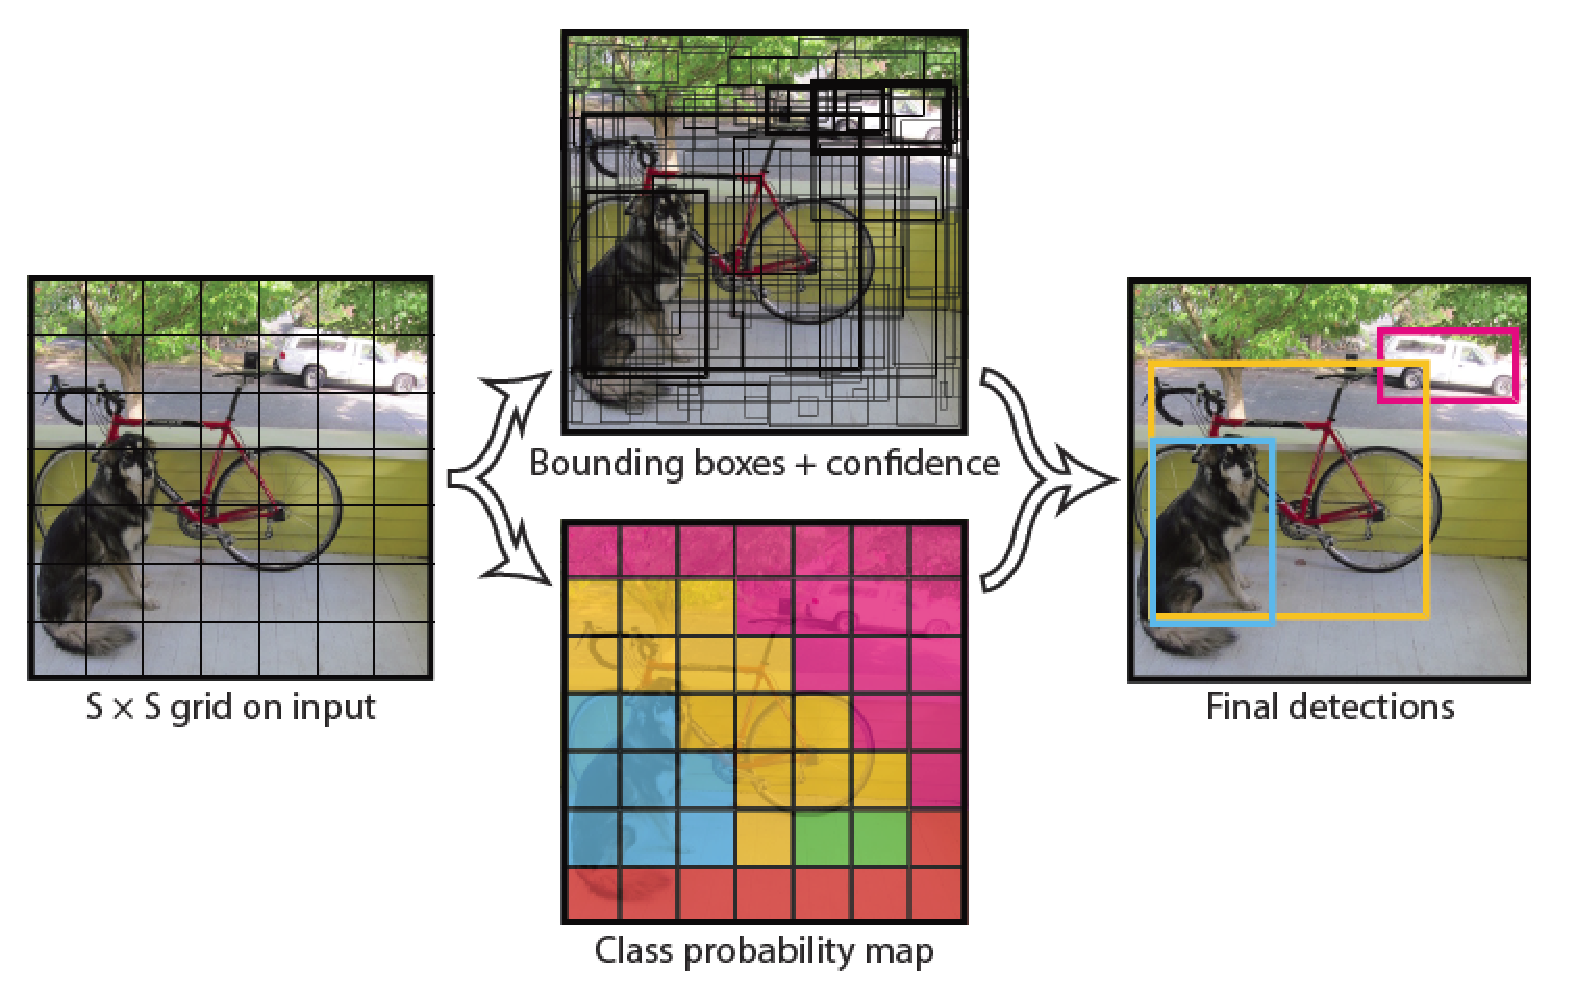
\includegraphics[height=75mm]{Figure/YOLO.eps}
	 \caption{物体検出YOLOの検出アルゴリズム}
	 \label{fig:f4}
\end{figure}
 物体の中心が特定のグリッドセル内に位置する場合、そのセルは物体を検出するように学習される。その後、各セルでバウンディングボックスが推定され、$B$個のバウンディングボックスに対してそれぞれ信頼スコアが予測される。
この信頼スコアは、特定のバウンディングボックスが物体を含む確率と、その精度を示す指標となる。\\
 次に、YOLOの損失関数について説明する。損失関数はネットワークの出力と正解ラベルとの誤差を計算する役割を担い、その最小化によってモデルの学習が進む。
損失関数は式(2.1)に示すように、物体の中心座標、バウンディングボックスの幅と高さ、物体の存在確率、クラス予測という4つの項目の誤差から構成される。

\begin{align*}
	\text{Loss} = 
	&\ \lambda_{\text{coord}} \sum_{i=0}^{S^2} \sum_{j=0}^{B} 1^{\text{obj}}_{ij} 
	\left[ (x_i - \hat{x}_i)^2 + (y_i - \hat{y}_i)^2 \right] \\
	&+ \lambda_{\text{coord}} \sum_{i=0}^{S^2} \sum_{j=0}^{B} 1^{\text{obj}}_{ij} 
	\left[ (2 - w_i \cdot h_i) \left[ (w_i - \hat{w}_i)^2 + (h_i - \hat{h}_i)^2 \right] \right] \\
	&- \sum_{i=0}^{S^2} \sum_{j=0}^{B} 1^{\text{obj}}_{ij} 
	\left[ \hat{C}_i \log(C_i) + (1 - \hat{C}_i) \log(1 - C_i) \right] \\
	&- \lambda_{\text{noobj}} \sum_{i=0}^{S^2} \sum_{j=0}^{B} (1 - 1^{\text{obj}}_{ij}) 
	\left[ \hat{C}_i \log(C_i) + (1 - \hat{C}_i) \log(1 - C_i) \right] \\
	&- \sum_{i=0}^{S^2} 1^{\text{obj}}_i \sum_{c \in \text{classes}} 
	\left[ \hat{p}_i(c) \log(p_i(c)) + (1 - \hat{p}_i(c)) \log(1 - p_i(c)) \right]
	\tag{2.1}
\end{align*}

ここで、$S^2$ はグリッドセルの総数を表し、$B$ は各グリッドセルで予測されるバウンディングボックスの数を示す。
また、$\lambda_{\text{coord}}$ と $\lambda_{\text{noobj}}$ は、それぞれ座標損失と物体が存在しない場合の信頼度損失に対応する重み付けパラメータを示す。
$(x_i, y_i)$ および $(w_i, h_i)$ は、バウンディングボックスの中心座標と幅・高さを示し、一方で $(\hat{x}_i, \hat{y}_i)$ および $(\hat{w}_i, \hat{h}_i)$ は、これらの推定値である。
$C_i$ および $\hat{C}_i$ は、物体が存在する信頼度スコアの真値と推定値を表す。
さらに、$p_i(c)$ および $\hat{p}_i(c)$ は、クラス $c$ に関する真値と推定値としてのクラス確率を意味する。


\subsection{6D姿勢推定}
6D姿勢推定ではGen6Dに基づき、画像マッチングおよび姿勢補正を行う。
画像マッチングでは、検出された物体の画像と参照画像を比較し、最も類似する画像を選択する。
この参照画像には、物体の姿勢データが含まれており、これを基に物体の初期姿勢を推定する。
参照画像の取得には、Colmapを用いて3D点群を再構築し、様々な角度からの参照画像に対する物体の初期姿勢データを取得する。
続いて、姿勢補正では、物体検出によって推定された物体の位置と、画像マッチングによって推定された回転を組み合わせて得られた初期の粗い物体姿勢をさらに精緻化するプロセスです。
具体的には、参照画像から6枚の近似視点を選択し、これらの平均と分散を計算して初期姿勢を補正し、最終的な姿勢を推定する。


\section{RGB-D画像に基づく配管6D姿勢推定}
\subsection{インスタンスセグメンテーション}
セグメンテーションは、画像からピクセル単位で対象物体を認識する手法であり、物体検出がバウンディングボックスの取得に留まるのに対し、より正確に物体の形状を特定できる。
RGB-D画像を活用することで、RGB画像からの色情報に加え、Depth画像からの距離情報も利用可能となり、配管の形状を詳細に把握し、姿勢推定の精度向上につなげる。
セグメンテーションを行う際には事前に配管画像のデータセットを用意し、学習を行うことで高い精度のセグメンテーションを実現する。
データセットには画像から接続部の箇所のみを切り取り、ラベル付けを行うことで、セグメンテーションの学習データを準備する。
配管の画像から検出クラスである曲管とT字管を全てセグメンテーションを行い、それぞれの位置や形状を抽出する。

\subsection{6D姿勢推定}
姿勢推定では、セグメンテーションで得られたそれぞれの配管に対して推定を行い、3次元空間上の位置情報と回転を求める。
姿勢推定には、事前に接続部の3Dモデルを用意することで、セグメンテーションで得られたオブジェクトの形状と照らし合わせることで、正確な姿勢推定を行う。
SAM-6Dによる姿勢推定では、物体表面の点とオブジェクトモデルの点を対応付けるポイントマッチングを用いる。
さらに、視野遮蔽(オクルージョン)が存在する場合でも精度を維持するため、仮想的な点であるバックグラウンドトークンを導入している。
これにより、欠損領域を含むシーンでも正確な姿勢推定を可能にする。


% 図\ref{fig:f3}は、配管の接続部であるT字管を検出した結果を示している。
% この例では、推定結果を示すバウンディングボックスを黄色で描画している。

% \begin{figure}[htbt]
% 	\centering
% 	 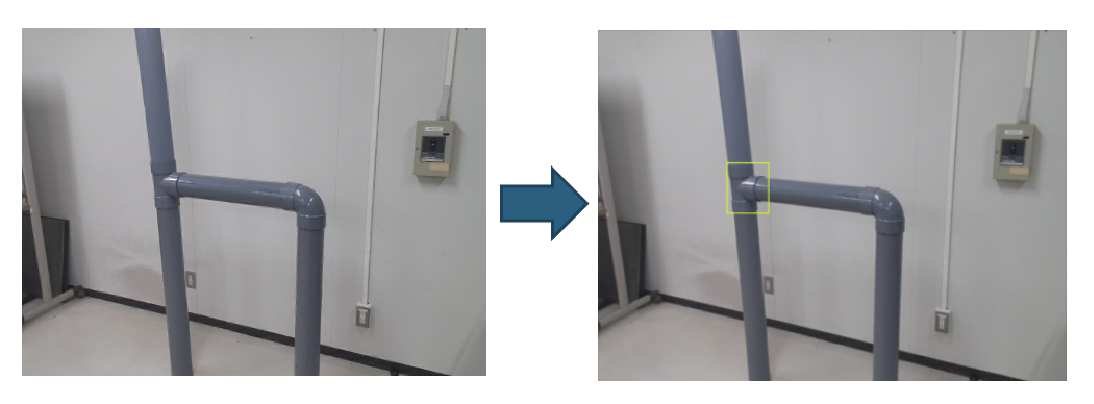
\includegraphics[height=52mm]{Figure/ex_YOLO.eps}
% 	 \caption{T字管を対象とした物体検出の可視化}
% 	 \label{fig:f3}
% \end{figure}

% また、物体検出をするにあたって、対象クラスの認識を向上させるためには学習を行う必要がある。

% \begin{figure}[htbt]
% 	\centering
% 	 \includegraphics[height=55mm]{Figure/label_detection.eps}
% 	 \caption{物体検出のラベリングの例}
% 	 \label{fig:f2}
% \end{figure}

% 図\ref{fig:f2}に物体検出のラベリングの例を示した。
% 学習にはラベル付きのデータセットが必要であり、配管の画像から曲管とT字管の接続部を切り取り、ラベル付けを行うことでデータセットを作成する。

% \section{全体構成}
% 配管6D姿勢推定とアイソメトリック図生成の手順について図\ref{fig:f1}に示す。
% \begin{figure}[htbt]
% 	\centering
% 	 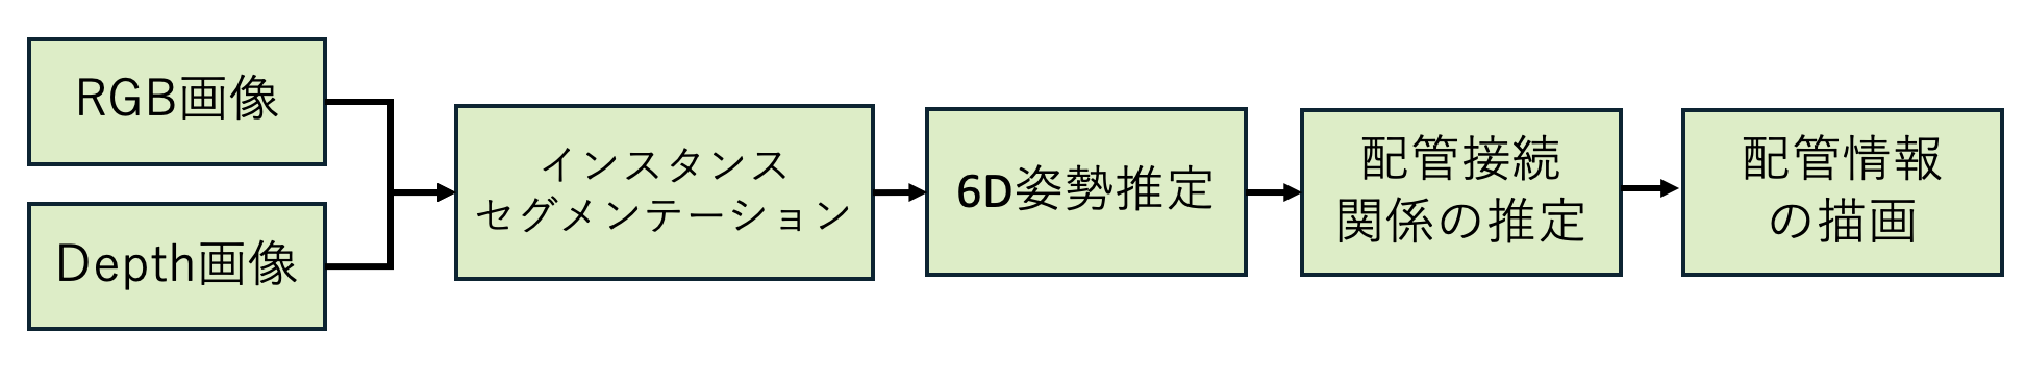
\includegraphics[height=25mm]{Figure/deep_flow.eps}
% 	 \caption{配管6D姿勢推定とアイソメトリック図生成の流れ}
% 	 \label{fig:f1}
% \end{figure}

% インスタンスセグメンテーション、姿勢推定、配管接続関係の推定、配管情報の描画の5つのステップに分類される。
% データ収集では、RGB-Dカメラを用いて配管の画像データを取得し、セアイソメ図生成で物体の形状を正確に把握し、高精度な姿勢推定を実現する。
% RGB画像からは色情報を、Depth画像からはピクセルごとの距離情報を取得することで、物体の形状を3次元空間で詳細に表現可能となる。
% 本手法では、配管6D姿勢推定のモデルとしてSAM-6Dを採用し、セグメンテーションと姿勢推定の2段階で処理を行う。







% \section{接続関係推定}
% アイソメ図を作成するには、接続部のペアを特定し、正確に配管を接続する必要がある。
% 配管間の接続関係を特定するために、接続部の方向ベクトルを計算し、そのベクトル間の角度差が小さい接続部をペアとして認識する。
% 曲管では出口が2つあるため2つの方向ベクトルを、T字管では3つの方向ベクトルを算出する。
% これらのベクトルの角度差が小さく、かつ距離が最も短い接続部をペアとして認識することで、接続関係を推定する。
% ただし、地面に接続している配管のようにペアが存在しない場合には、ペアマッチングを適用しない。

% \section{配管経路の探索} 
% 接続された配管の経路を効率的に探索するため、深さ優先探索(Depth First Search, DFS)アルゴリズムを使用する。
% DFSは、グラフ構造内のノードを一つの経路で可能な限り深く進み、行き止まりに達した際に戻って別の経路を探索するアルゴリズムである。
% この手法により、すべての接続部を効率的に訪問し、再帰的に探索を進めることが可能となる。
% 探索の起点は最も左端に位置する配管とし、接続情報に基づいて配管を順次描画する。

% \subsection{アイソメ図の描画} 
% アイソメ図の描画には、Pythonのezdxfライブラリを使用する。
% ezdxfはDXFファイルの作成に特化しており、直線や円弧などの描画が可能である。
% 配管の寸法情報は、カメラ座標系で取得した3次元位置データを基に計算される。
% 配管経路探索で得られた接続情報をもとに、ezdxfを用いて正確なアイソメ図を描画する。
% この方法により、配管システムの構造を視覚的に表現する図面を効率的に作成することができる。







% データ収集において、本研究では、RGB-D カメラ(Intel Realsense D435i)を用いて、配管データを収集した。
% RGB-D カメラは、3D レーザースキャナーと比べ、圧倒的に安価である。また、軽量化及び小型化され、複雑な配 管環境に最適だと考えられる。
% RGB-D カメラで収集したデータは、カラー画像(RGB)だけでなく、対象までの 距離、或は深度データ(D)も取得できる。対象までの距離に基づき、三次元点群を得ることができる。
% すなわち、 カラー画像の各ピクセルは、一つの三次元点群に対応するということである。
% データ処理において、本研究では、データ処理と認識を同時に行うという手法を提案した。
% それぞれの深度画像 から得た三次元点群を合併し、配管点群モデルを構築する。一方、深層学習による画像セグメンテーションを行う ことで、予測マップを求める。
% 最後に、データ統合では、配管点群モデルに深層学習での予測マップを付けることで、ラベル付きの配管点群モ デルを得ることができ、三次元配管認識を実現できる。


% \begin{figure}[htbt]
% 	\includegraphics[height=65mm]{flow2.eps}
% 	\caption{RGB-Dカメラを用いた深層学習による配管6D姿勢推定までの手順}
% 	\label{fig:f2}
% \end{figure}




% \section{アイソメ図変換方法}
% アイソメ図作成には配管の特徴を活かした効率的な手法を提案する.図2.2に一部配管の例を示す.
% 一般的な配管は両端部分の曲管やT字管などのつなぎ目を除くと直管であるという特徴がある.そのため,両端の曲管がどの方向を向いているのかを推論できれば向かい合っている曲管のペアを見つけられ,その間を直線で結ぶことで
% アイソメ図を描画することができる.そのため,本研究においては配管全体を認識するのではなく,配管のつなぎ目である曲管及びT字管を物体検出と姿勢推定を用いて推論する.

% \begin{figure}[htbt]
% 	\centering
% 	 \includegraphics[height=55mm]{pipe.eps}
% 	 \caption{配管の検出例}
% 	 \label{fig:f2}
% \end{figure}


% \section{データセット収集}
% 深層学習による認識ネットワークにはデータセットの数量が多いほど精度とロバスト性が向上する.
% それは様々な場面での配管の写真を学習することによってどの環境においても対応できる汎用性が高まることを意味している.本研究使用するデータセットの一部を図3.2に示す.
% 配管には曲管やT字管や直管が含まれており,この画像内の中から曲管とT字管を全て認識できることを目標とする.また,Depth画像の有効性を示すためにテスト画像では
% 暗闇の中に配管を設置したデータセットを用意した.Depth画像は光の影響を受けにくいことから,暗闇の中でも配管を認識できるかを検証する.\\
% 収集したデータはラベリング作業を行う.これは深層学習するにおいての正解データとして,予め画像内のどの部分が曲管又はT字管であるかをアノテーションする必要がある.
% 本研究では配管画像に対して曲管,T字管の二つのクラスに分けてラベリング作業を行った.

% 6D姿勢推定のデータセットにはColmapを使用して点群データを取得する.Colmap2D画像から点群を再構築するために使用されるソフトウェアである.
% この2D画像は異なる視点から撮影された同じオブジェクトの画像を複数枚利用することで3次元情報を復元することができる.
% そのため,本研究では曲管とT字管の周囲をそれぞれ撮影し,Colmapを使用することで点群データを取得した.
% 図3.6では姿勢推定を行った後,得られた出力の評価を行う際に使用する.
% しかし,点群データを取得してもColmapで生成されたデータには距離情報が含まれていないため,別途Depth画像を使用してアイソメ図作成の際に使用しなければいけない.
